\subsection{Deep Learning}

Information about deep learning (what is deep learning):
Deep learning is a branch of machine learning. The main difference between the use of ML and deep learning, is that first one is not suitable for handle raw data form. Instead a machine learning system often needs a feature extractor, that will generate a feature vector from the data that can be used as an input for the ML system. \citep{LeCun2015}
Deep learning is based on different techniques that makes it able to handle that data in its raw form, mainly because of it’s structure. \citep{LeCun2015, Schmidhuber2015}. Because of this the system will automatically detect the necessary representations needed for classification and detection \citep{LeCun2015}. The neural network consists of different layers, that can be divided into a input-layer and an output-layer, with one or more hidden layers in between \citep{LeCun2015, Schmidhuber2015}. The key aspect of these layers is that the features are not defined by programmers, but they are found and learned from raw data using a general – purpose learning procedure. \citep{LeCun2015} An example of the structure can be seen in \autoref{fig:NN_structure}.   


\begin{figure} [H]
\centering
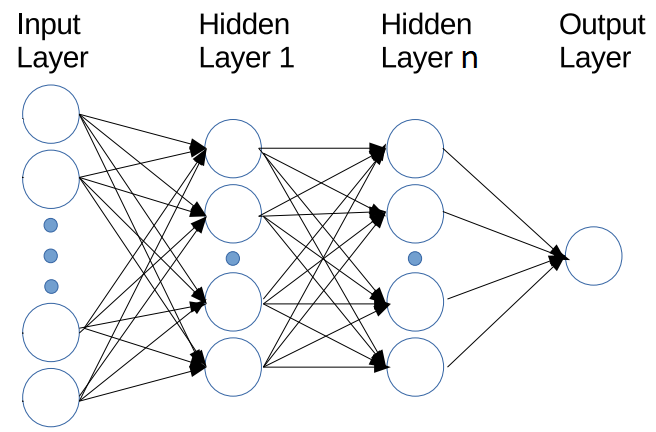
\includegraphics[width=1\textwidth]{figures/NN_structure}
\caption{BLABLABLA}
\label{fig:NN_structure}  
\end{figure}


The different layers consist of a series of processors/Neurons/Nodes, where each node is connected to one or several other nodes from a different layer. In the input-layer the nodes are fed with the data that the system is given. The second layer will then receive the output from the previous layer, and this processes continues through the layers until the output-layer is reached. \citep{Schmidhuber2015} An example of how the hidden layers affect the data e.g. an image can be explained as follows:  
Firstly, the system detects minor changes like edges. Secondly, the edges are compared and put together to make up different kind of shapes. In the third hidden layer, it will be further combined to make up an object that can be identified. \citep{LeCun2015}

\subsection{Supervised Learning}
Supervised learning is the most common way of training in machine learning \citep{LeCun2015}. When using this method the system is trained with labeled data, where the generated output can be compared with an expected output, and thereby see how accurate the system is. By adjusting weights inside the neural network it is possible to fit the model better to the training data, and thereby increase its accuracy and reduce error. \citep{LeCun2015} Supervised learning is mostly associated with classification, regression, and ranking problems \citep{Mehryar2012}.

\subsection{Unsupervised Learning}
Differently from supervised learning in this scenario the input is received with unlabeled data and the predictions are made for all unseen points \citep{Mehryar2012}. An example of an unsupervised learning algorithm is clustering, where the unlabeled dataset goes through a classification, and split into different classes. \citep{Goodfellow2016} 

\subsection{Semi-supervised Learning}
In this scenario, the learner is receiving both labeled, unlabeled data and then it makes prediction for all unseen points. It is used mainly when the labeled data is hardly collected and unlabeled data is easily reachable \citep{Mehryar2012}.

\subsection{Convolutional Neural Networks}
CNN perform highly in several tasks, including digit recognition, image classification and face recognition. The key aspect of CNNs is to automatically learn a complex model that is able to extract visual features from the pixel-level content. Operations like filtering, local contrast normalization, nonlinear activation and local pooling are being used \citep{Acquarelli2017}.
CNNs are a feed – forward models that maps input data with a set of suitable outputs. 
Accuracy and performance rely on large training datasets and training procedure based on back-propagation with optimization algorithm such as gradient descent \citep{Acquarelli2017}.

\subsection{Backpropagation}
Back – propagation is a popular learning algorithm in convolutional neural network. It is valuable because of the simplicity, computationally efficient and because it usually works \citep{Bengio2012}.
Basic idea behind it is to minimize the overall output error as much as possible during the learning stage. This algorithm process is divided in two main stages: forward and backward. In the first process (forward), the BP architecture is described as  the inputs and weights multiplication of each neuron (separate input) summed with biases \citep{Hameed2016}. 

\begin{comment}
It is defined by:
%H(j)=b_in+∑_(i=1)^N▒〖x_i w_ij 〗
Where: x – the inputs, i – neurons, w_ij – weights, j – neurons for hidden layer, b_in – biases
\end{comment}

In the backward process, weights will be updated to minimize the error between target and output layer.
This process will be applied until optimal weights with minimum error is reached \citep{Hameed2016}.


